\documentclass{article}

\usepackage{mathtools}
\usepackage{amssymb}
\usepackage{graphicx}
\usepackage{subfiles}
\usepackage{verbatim}
\usepackage{physics}
\usepackage{hyperref}
\usepackage[margin=1in]{geometry}

\hypersetup{
    colorlinks=true,
    linkcolor=black,
    filecolor=magenta,      
    urlcolor=cyan}

\newcommand{\parti}[2]{ \frac{\partial#1}{\partial#2} }
\newcommand{\errorterm}[2]{ \left(\frac{\partial#1}{\partial#2} \Delta#2\right)^2 }
\newcommand{\tento}[1]{ \times\@ 10^{#1} }
\newcommand{\secs}{\mbox{s}}
\newcommand{\Hz}{\mbox{Hz}}
\newcommand{\kgs}{\mbox{kg}}
\newcommand{\mets}{\mbox{m}}
\newcommand{\cms}{\mbox{cm}}
\newcommand{\newt}{\mbox{N}}
\newcommand{\amps}{\mbox{A}}
\newcommand{\joules}{\mbox{J}}
\newcommand{\volts}{\mbox{V}}
\newcommand{\tesla}{\mbox{T}}
\newcommand{\emratio}{\mbox{C/kg}}
\newcommand{\psid}{\dot{\psi}}
\newcommand{\psidd}{\ddot{\psi}}
\newcommand{\bunits}{\mbox{kgm}^2\mbox{s}^{-1}}
\newcommand{\avgemratio}{\bar{\frac{e}{m_e}}}
\newcommand{\rbrak}[1]{\left(#1\right)}
\newcommand{\sbrak}[1]{\left[#1\right]}
\newcommand{\cbrak}[1]{\left\{#1\right\}}
\newcommand{\abrak}[1]{\left<#1\right>}
\newcommand{\bbrak}[1]{\left|#1\right|}
\newcommand{\rdot}{\dot{r}}
\newcommand{\rddot}{\ddot{r}}
\newcommand{\thetadot}{\dot{\theta}}
\newcommand{\thetaddot}{\ddot{\theta}}
\newcommand{\phidot}{\dot{\phi}}
\newcommand{\phiddot}{\ddot{\phi}}

\newcommand{\class}{COMP 4911}
\newcommand{\examnum}{Bookdex: Design Document}
\newcommand{\examdate}{\today}
\newcommand{\yourname}{Sawyer Stanley}
\newcommand{\studentid}{0289276}

\begin{document}
\pagestyle{plain}

\vspace*{\fill}
\begin{center}
    \yourname\\
    \studentid\\
    \class\\
    \examnum\\
    \examdate\\
\end{center}
\vspace*{\fill}

\thispagestyle{empty}
\newpage
%--

\section{Preface}\label{sec:preface}
The following document contains justifications annd explainations of the decisions made during the development of Bookdex.

Acronyms are often used throughout this document. Common acronyms include:

\begin{itemize}
    \item \textbf{TDS}: Tabular Data Stream Protocol
    \item \textbf{GUI}: Graphical User Interface
    \item \textbf{UML}: Unified Modeling Language
    \item \textbf{I/O or IO}: Input/Output
\end{itemize}

\section{Development Plan}\label{sec:plan}

    \begin{figure}[h]\label{fig:gantt}
        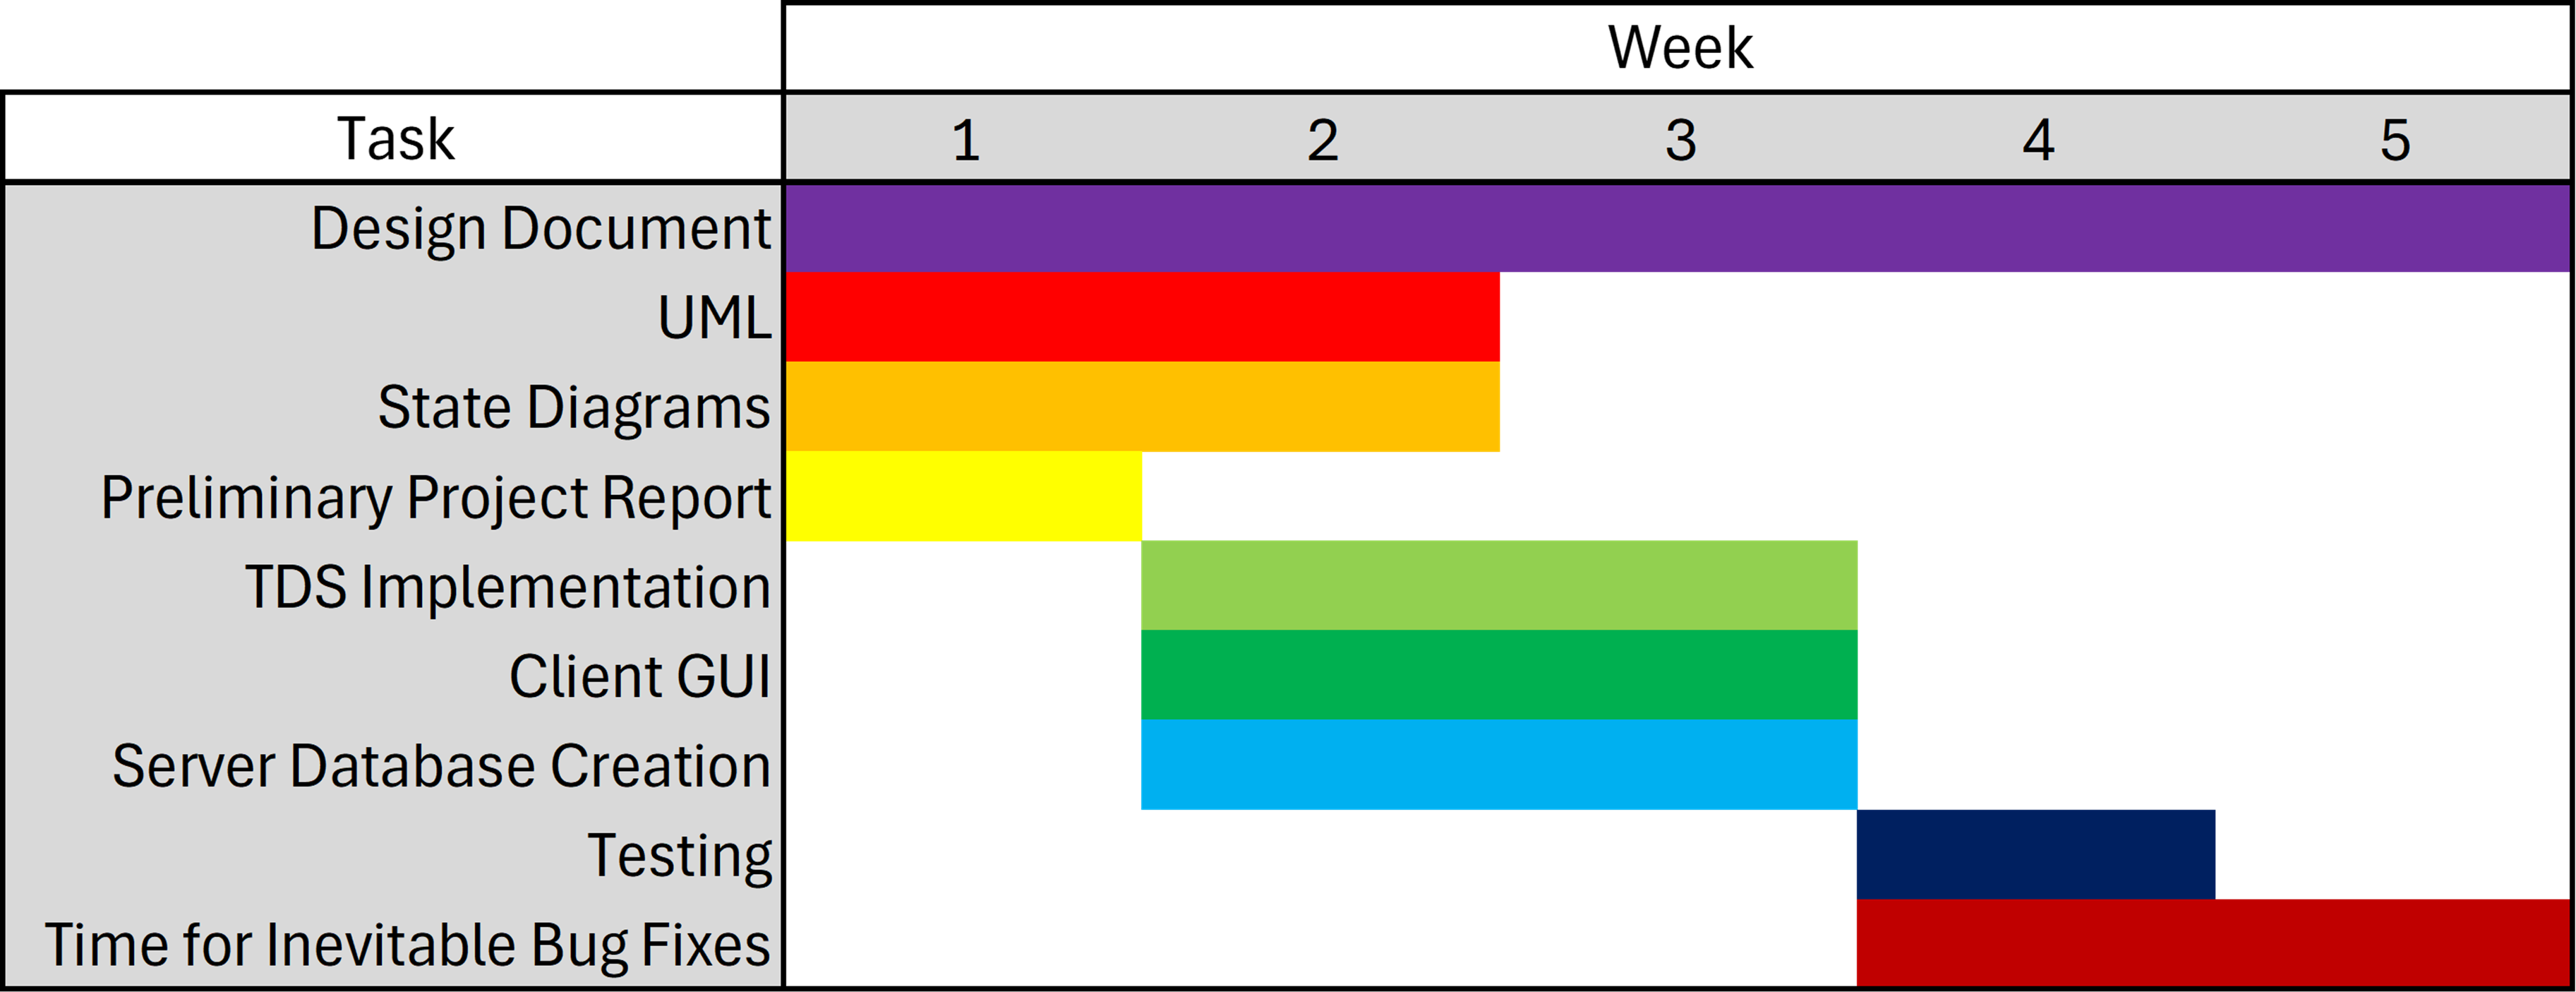
\includegraphics[width=0.9\textwidth]{gantt_chart.png}
        \caption{Gantt chart outline for the development plan for Bookdex.}
    \end{figure}

\section{UML Class Diagrams}\label{sec:uml}
    Recognizing that this is difficult to see, .png versions have been uploaded to the \href{https://github.com/SawyersCoding/bookdex/tree/main}{GitHub repository} for for this project.

    The (current) UML class diagram for the TDS protocol is shown in Figure~\ref{fig:tdsuml}.

    \begin{figure}[h]\label{fig:tdsuml}
        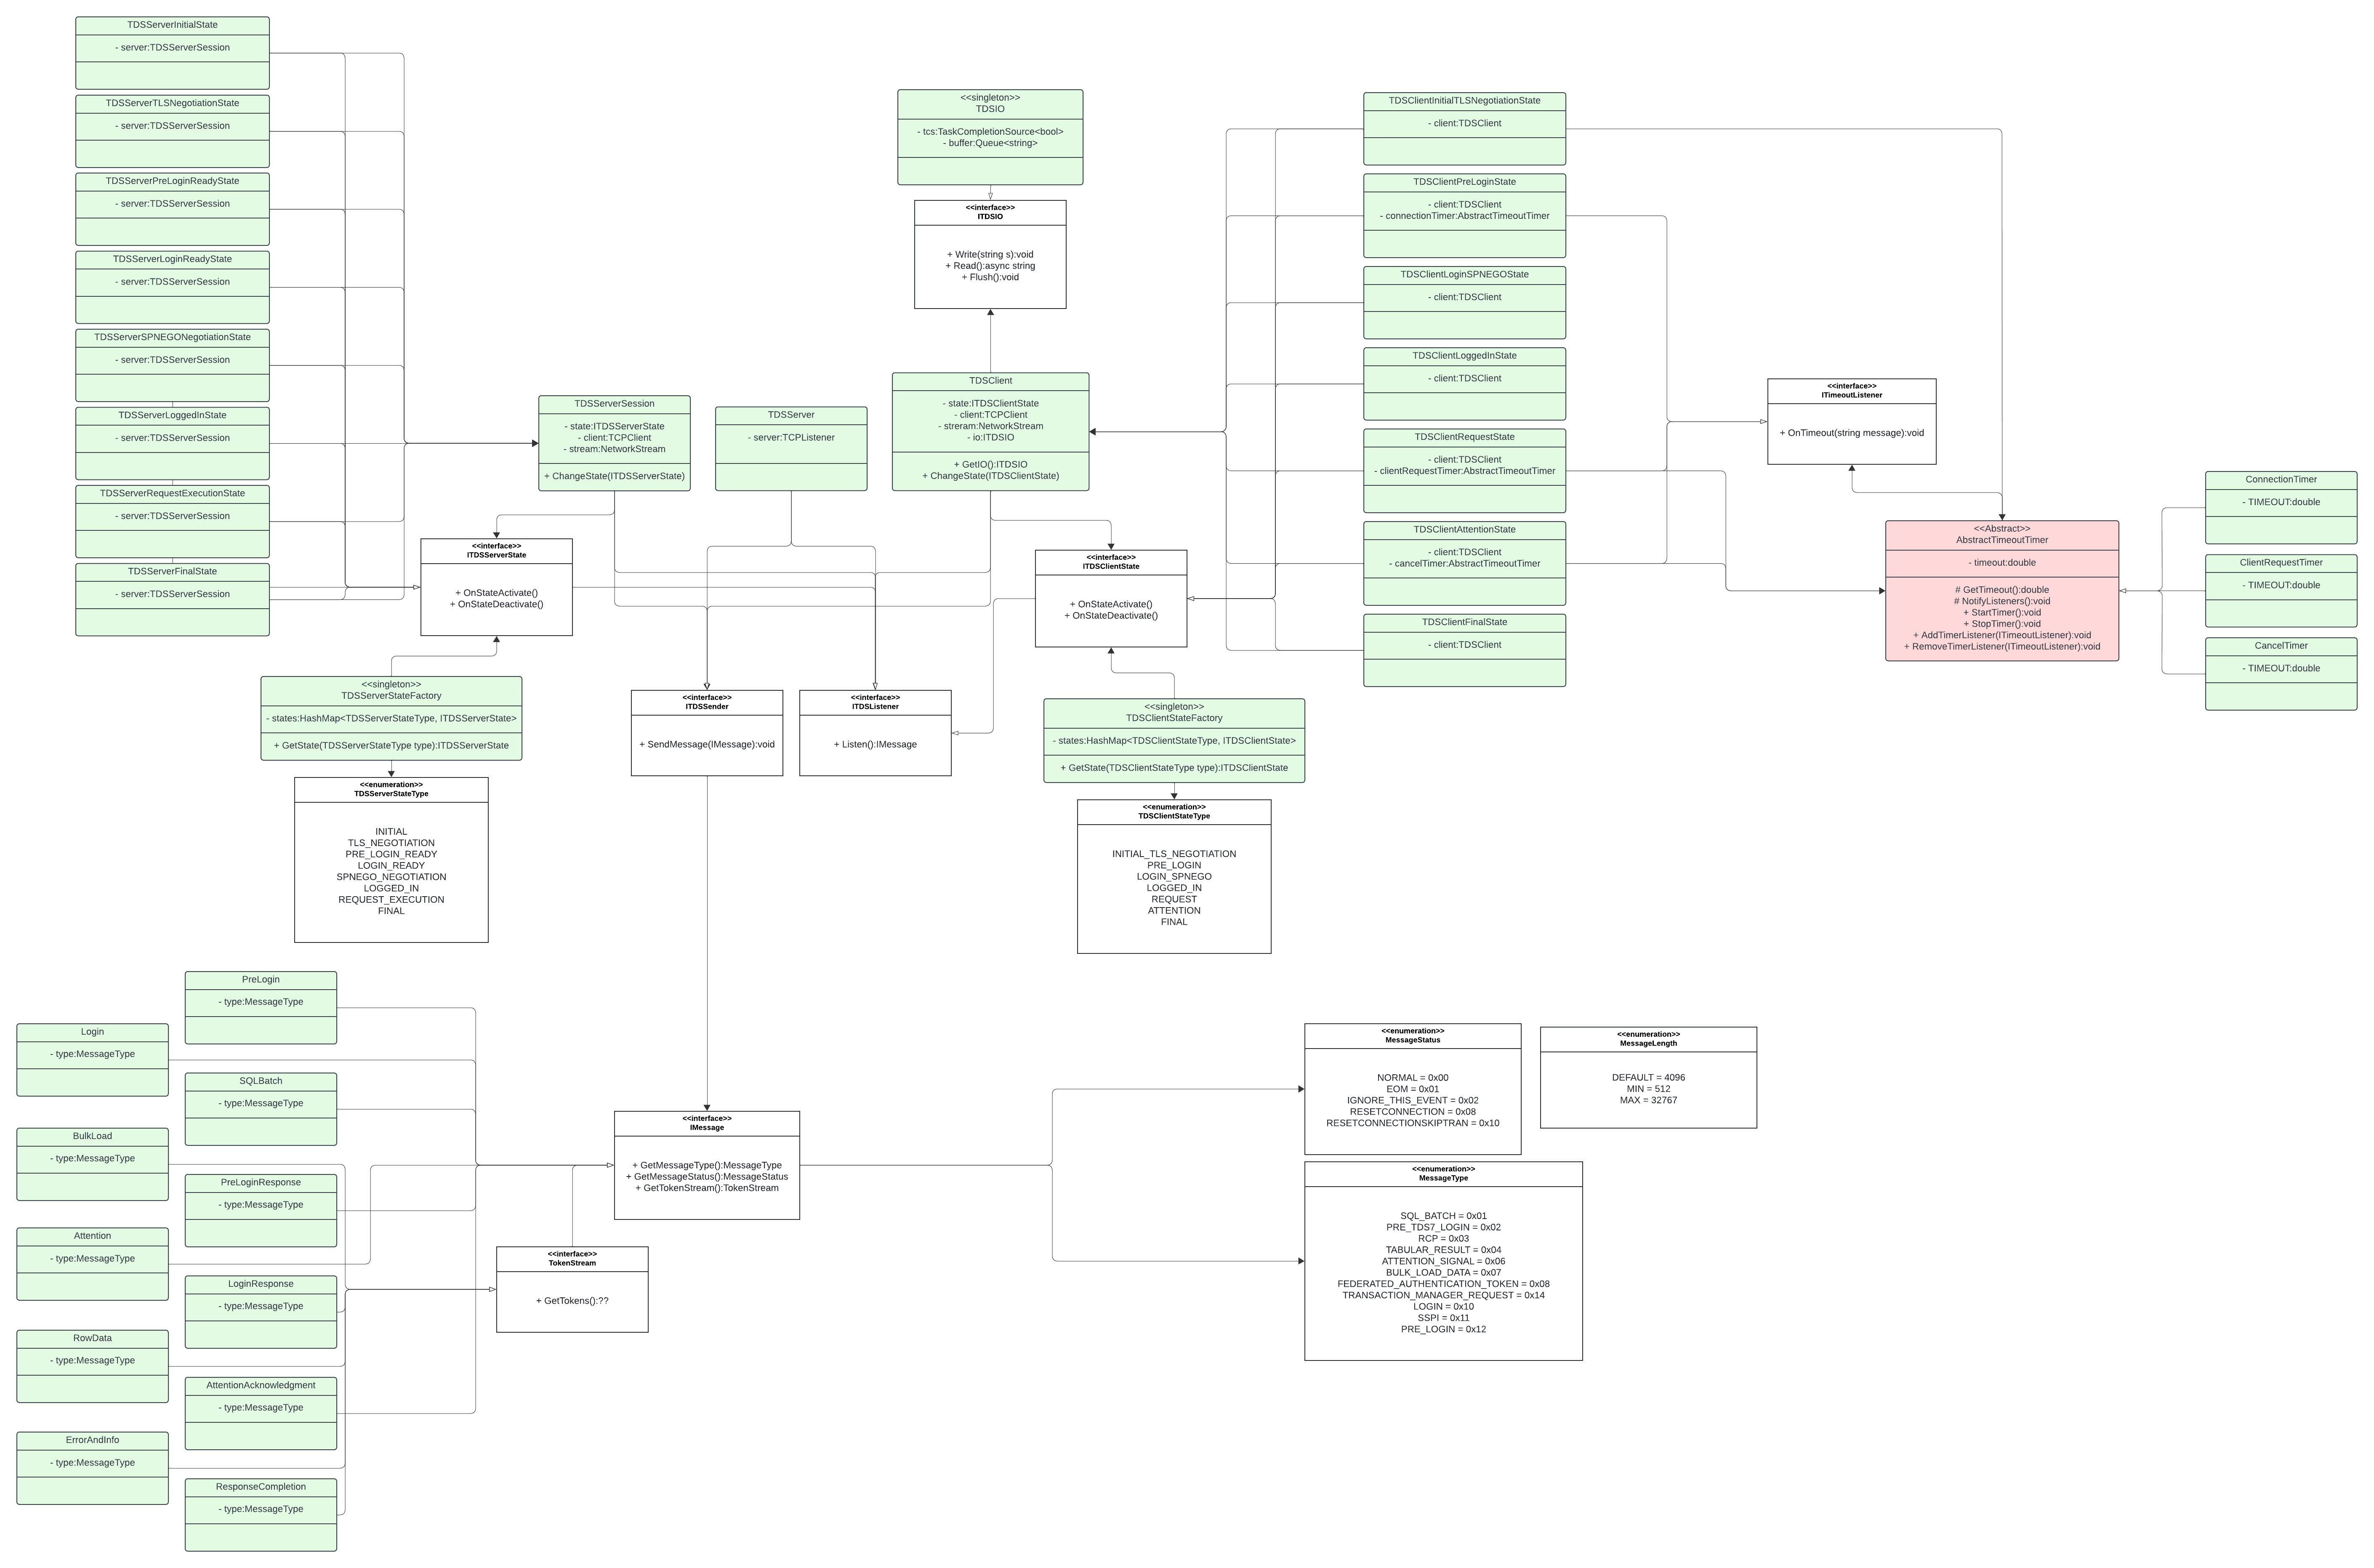
\includegraphics[width=0.9\textwidth]{uml_tds.png}
        \caption{UML diagram outlining the structure of the TDS protocol implementation.}
    \end{figure}

% \section{State Diagrams}\label{sec:state}

\section{Retrospectives}\label{sec:retro}
    \subsection{Week 1}\label{sec:retro:week1}
        This week began with work on the UML class diagram for the TDS protocol. During its creatation, reference \textbf{INSERT TDS MANUAL REFERENCE} was consulted regularly. This slowed progress as the TDS protocol is nuanced. For example, there are a handful of different types of tokens to be used when transmitting a token stream, each with their own rules. To add to this, not all messages transmitted are token streams. Decomposing the intricate case-work into meaningful classes has helped with understanding the protocol overall.

        As seen in Section~\ref{sec:uml}, various timers are used by the client to ensure the client is not waiting too long for a response from the server. It's important to note that TDS does not require these timers. Initial implementation will omit these timers for simplicity's and time's sake.

\section{Decisions}\label{sec:dec}
    While not every decision is outlined in this section, decisions that were made unexpectedly or creatively are included.

    \subsection{Client-side I/O}\label{sec:dec:clientio}
        As seen in Section~\ref{sec:uml}, the states in which a TDSClient can exist handle the Listen() operation. Initially, Listen() was intended for receiving packets send from the server to the client. However, when in the TDSClientLoggedInState, the user should be able to enter a request to be sent to the server before the client listens for a response. The definition of Listen() was then expanded to include ``listening'' for input from the user.

        Anticipating user input to come from various input streams, I planned to create a custom input stream to which all input could be written and from which the program could consistently read. Upon researching halting the program to wait for input on said stream, I began to fear I had gone astray. Instead, I opted to create custom I/O, namely, TDSIO (Tabular Data Stream Protocol Input/Output). Now, when a user writes to the ``input stream'', their input is enqueued to a queue of inputs. When these inputs are flushed, a notification of a complete task will be sent to the listening TDSClientLoggedInState. The queue is then emptied and the TDSClientLoggedInState can do with the inputs what it will. This way, implementation of a view, whether GUI or console, will be supported (I think).

% \section{User Guide}\label{sec:userguide}

\end{document}
